% article example for classicthesis.sty
\documentclass[10pt,a4paper]{article} % KOMA-Script article scrartcl
\usepackage{lipsum}     %lorem ipsum text
\usepackage{titlesec}   %Section settings
\usepackage{titling}    %Title settings
\usepackage[margin=10em]{geometry}  %Adjusting margins
\usepackage{setspace}
\usepackage{listings}
\usepackage{amsmath}    %Display equations options
\usepackage{amssymb}    %More symbols
\usepackage{xcolor}     %Color settings
\usepackage{pagecolor}
\usepackage{mdframed}
\usepackage[spanish]{babel}
\usepackage[utf8]{inputenc}
\usepackage{longtable}
\usepackage{multicol}
\usepackage{graphicx}
\graphicspath{ {./Images/} }
\setlength{\columnsep}{1cm}

% ====| color de la pagina y del fondo |==== %
\pagecolor{black}
\color{white}



\begin{document}
    %========================{TITLE}====================%
    \title{\rmfamily\normalfont\spacedallcaps{ Demostracion  }}
    \author{\spacedlowsmallcaps{Rodrigo Castillo}}
    \date{\today} 
    
    \maketitle
     

     % ====| Loguito |==== %
    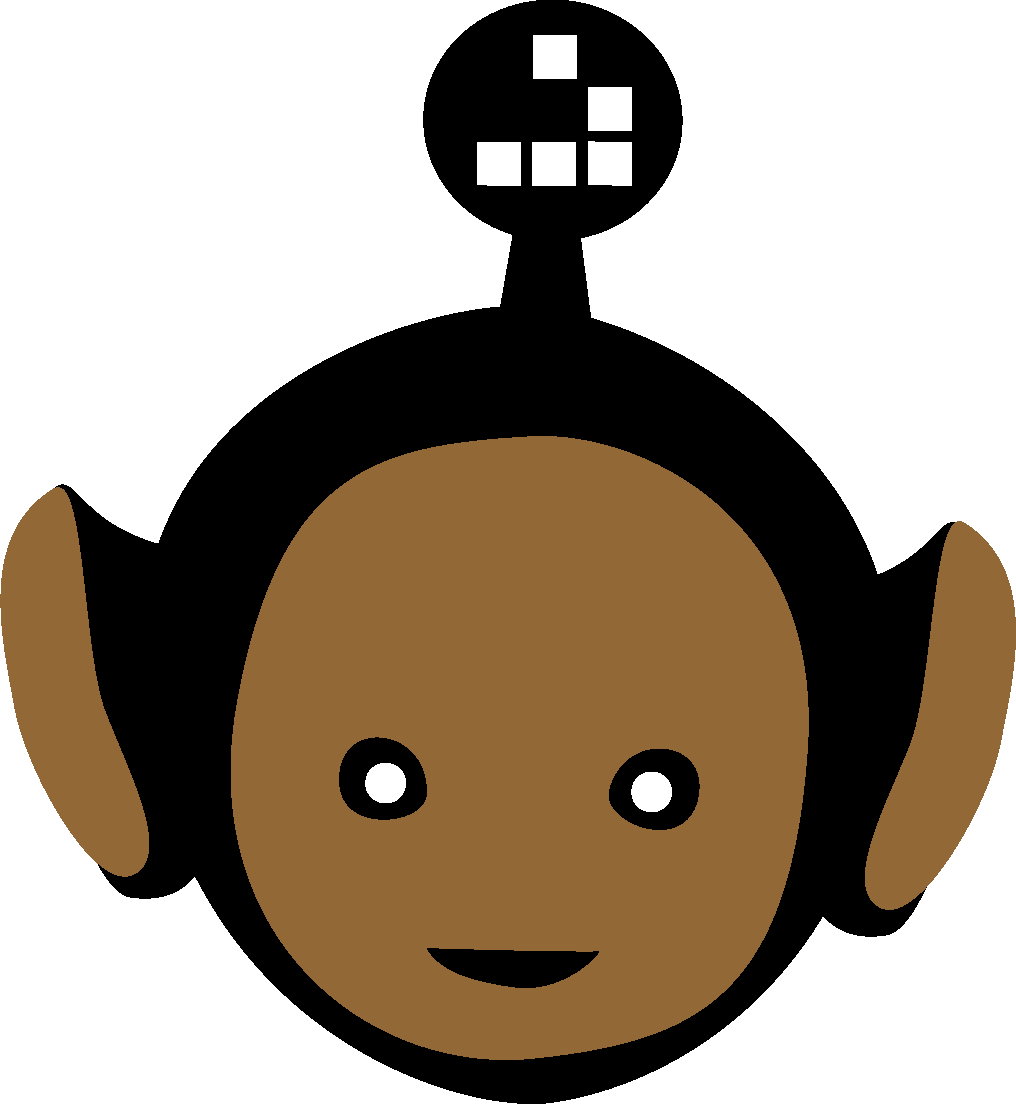
\includegraphics[width=0.1\linewidth]{negro_cara.png}
    %=======================NOTES GOES HERE===================%
    \\
    dado un conjunto $ A  $  una particion $ {A_1 , A_2 ... A_n}  $  es una coleccion de subconjuntos tales que $ A  $ satisface que:
    \begin{itemize}
        \item {$A_i != \emptyset$} 
        \item {se tiene que $ \cup A_i = A   $ } 
        \item {$ A_i \cap A_j   = \emptyset$ para todos $ i != j  $  } 
    \end{itemize}	
    \section{Teorema}
        Sea R una relación de equivalencia sobre un conjunto A. Entonces la
        colección de clases de equivalencia respecto a R es una partición de
        A.
        Por otro lado, dada una partición {A 1 , A 2 , . . .} de A existe una
        (única) relación de equivalencia R sobre A cuya clases de
        equivalencia son exactamente A 1 , A 2 , . . ..
    \section{Demostracion}
        Supongamos que R es una relación de equivalencia sobre A, por lo tanto
        R es simétrico, transitivo y reflexivo. 
        \\Sean $ A_i , A_j  $ elementos de $ R  $ 
        \item {1 : $ A_i != \emptyset$ }  
        \\ supongamos que $ A_i \subset A  $  pero $ A_i = \emptyset  $  \\
        por lo tanto bla bla bla
        \item {2: $ A \cup A_i  != \emptyset $  }\\
            \begin{enumerate}
                
            \end{enumerate}
            

        \item {3: $ A_i \cap A_j = \emptyset \implies i != j  $ }
            \\ 
            Supongamos que $ A_i \cap A_j = \emptyset   $ pero $ i = j  $  
            \\ por lo tanto existe $ a \in A_i  $  tal que $ a \in  A_j  $ 
            \\ como R es reflexivo tenemos que $ a \in  A_i  $ y $ a \in A_j  $ 
            \\ por lo tanto $ A_i \cap A_j != \emptyset  $  
        
        
        
    
    







    %=======================NOTES ENDS HERE===================%
    
    % bib stuff
    \nocite{*}
    \addtocontents{toc}{\protect\vspace{\beforebibskip}}
    \addcontentsline{toc}{section}{\refname}    
    \bibliographystyle{plain}
    \bibliography{../Bibliography}
\end{document}
